%% Data & Knowledge Engineering / Elsevier CAS supplementary package.
%% SC-FMA: Structurally-Calibrated Functional Attribution for Knowledge Curation
\documentclass[a4paper,fleqn]{cas-sc}

\usepackage[numbers,sort&compress]{natbib}
\usepackage{amsmath}
\usepackage{booktabs}
\usepackage{array}
\usepackage{graphicx}
\usepackage{xurl}
\usepackage{amsthm}
\newtheorem{theorem}{Theorem}[section]
\newtheorem{lemma}[theorem]{Lemma}
\newtheorem{corollary}[theorem]{Corollary}
\usepackage{algorithm}
\usepackage{algpseudocode}
\usepackage{multirow}
\usepackage{makecell}
\usepackage{hyperref}
\hypersetup{colorlinks=true,linkcolor=blue,citecolor=blue,urlcolor=blue}


\begin{document}
\let\WriteBookmarks\relax
\def\floatpagepagefraction{1}
\def\textpagefraction{.001}
\pagenumbering{arabic}

\shorttitle{Supplementary Material}
\shortauthors{Ma and Wang}

\title[mode=title]{Supplementary Material for Structurally-Calibrated Functional Attribution for Audit Prioritization in Knowledge-Intensive Reasoning}

\author[1]{Haoran Ma}
\ead{mahaoran0000@foxmail.com}

\author[1,2]{Ningning Wang\corref{cor1}}
\ead{wangningning@bistu.edu.cn}

\cortext[cor1]{Corresponding author.}

\affiliation[1]{organization={College of Management Science and Engineering, Beijing Information Science and Technology University},
            city={Beijing},
            postcode={102200},
            country={China}}

\affiliation[2]{organization={Institute of Information Systems, ESG Intelligent Application Innovation Research Center},
            city={Beijing},
            postcode={102200},
            country={China}}

\begin{abstract}
This supplementary material contains extended proofs, additional controlled-stage results, implementation details, and reproducibility notes separated from the main manuscript. The synthetic labels discussed here are controlled proxy labels for representation-behavior analysis, not external ground truth.
\end{abstract}

\begin{keywords}
supplementary material \sep structural calibration \sep reproducibility \sep knowledge graph diagnostic
\end{keywords}

\maketitle

\appendix
\makeatletter
\renewcommand{\thetable}{\@Alph\c@section.\arabic{table}}
\renewcommand{\thefigure}{\@Alph\c@section.\arabic{figure}}
\renewcommand{\thealgorithm}{\@Alph\c@section.\arabic{algorithm}}
\renewcommand{\theequation}{\@Alph\c@section.\arabic{equation}}
\makeatother
% ===================================================================

\section{Extended Proofs and Derivations}
\label{app:proofs}

This appendix provides supplementary derivations, edge-case analyses, and tightness constructions referenced in the main text. Full proofs of the variance-reduction and bottleneck-protection theorems, the bottleneck tightness construction, and SLSQP convergence diagnostics are provided in the subsections below.

\subsection{KKT Conditions for the SCU Objective}
\label{app:kkt}

The Karush--Kuhn--Tucker (KKT) conditions for the SCU constrained optimization problem (Eqs.~1--2) are:

\begin{align}
\frac{\partial L}{\partial w_i}\bigg|_{\mathbf{w}^*} - \mu_i^* - \lambda^* &= 0, \quad \forall i \\
\mu_i^* &\ge 0, \quad \forall i \\
\mu_i^*(w_i^* - \varepsilon) &= 0, \quad \forall i \\
w_i^* &\ge \varepsilon, \quad \forall i \\
\sum_{i=1}^k w_i^* &= 1.
\end{align}

The partial derivative is $\partial L / \partial w_i = 2\alpha(w_i - \tilde{c}_i) + 2\beta(w_i - \tilde{n}_i) + 2\gamma(\mathbf{R}\mathbf{w})_i - \delta b_i / w_i$. The multiplier $\lambda^* \in \mathbb{R}$ (unrestricted) captures the equality constraint; $\mu_i^* \ge 0$ enforce the floor constraints. By complementary slackness, $\mu_i^* > 0$ only when $w_i^* = \varepsilon$.

\subsection{Derivation of the Variance Reduction Bound}
\label{app:variance-derivation}

The full algebraic derivation is provided below. The key steps are: (i) the two-term objective $L_2(\mathbf{w}) = \alpha\|\mathbf{w} - \tilde{\mathbf{c}}\|_2^2 + \beta\|\mathbf{w} - \tilde{\mathbf{n}}\|_2^2$ has unconstrained minimizer $\hat{\mathbf{w}} = (\alpha\tilde{\mathbf{c}} + \beta\tilde{\mathbf{n}})/(\alpha+\beta)$; (ii) variance decomposes as $\operatorname{Var}(\hat{\mathbf{w}}) = (\alpha/(\alpha+\beta))^2\operatorname{Var}(\tilde{\mathbf{c}}) + (\beta/(\alpha+\beta))^2\operatorname{Var}(\tilde{\mathbf{n}}) + 2\alpha\beta/(\alpha+\beta)^2\operatorname{Cov}(\tilde{\mathbf{c}}, \tilde{\mathbf{n}})$; (iii) since $\operatorname{Cov}(\tilde{\mathbf{c}}, \tilde{\mathbf{n}}) \approx 0.05$--$0.09$ and $\operatorname{Var}(\tilde{\mathbf{n}}) \ll \operatorname{Var}(\tilde{\mathbf{c}})$, the dominant shrinkage factor is $\alpha/(\alpha+\beta)$; (iv) projection onto the simplex $\mathcal{W}$ is non-expansive in variance~\cite{wang2013projection}, yielding the stated bound.

\subsection{Tightness Construction for Bottleneck Lower Bound}
\label{app:bottleneck-tightness}

The explicit tightness construction for the bottleneck lower-bound theorem is provided below.

Substituting $w_2 = 1 - w_1$:
\begin{equation}
L(w_1) = (\alpha+\beta)(w_1^2 + w_1^2) - \delta\log(w_1) = 2(\alpha+\beta)w_1^2 - \delta\log(w_1).
\end{equation}

The first-order condition:
\begin{equation}
\frac{dL}{dw_1} = 4(\alpha+\beta)w_1 - \frac{\delta}{w_1} = 0 \implies w_1^* = \sqrt{\frac{\delta}{4(\alpha+\beta)}}.
\end{equation}

Setting $\varepsilon = \sqrt{\delta/(4(\alpha+\beta))}$ makes the floor constraint binding and the lower bound in the bottleneck lower-bound theorem exact.

\subsection{Monotonicity Violation under Redundancy}
\label{app:monotonicity-redundancy}

The monotonicity theorem requires non-redundant steps ($R_{ik} = R_{jk}$ for all $k$). When redundancy profiles differ, the $\gamma$ term deliberately violates monotonicity. We illustrate with a minimal example.

Consider $k = 2$ with $\tilde{\mathbf{c}} = (0.6, 0.4)^\top$, $\tilde{\mathbf{n}} = (0.5, 0.5)^\top$, $b_1 = b_2 = 0$, and:
\begin{equation}
\mathbf{R} = \begin{bmatrix} 1.0 & 0.9 \\ 0.9 & 1.0 \end{bmatrix}.
\end{equation}
Here $\tilde{c}_1 > \tilde{c}_2$ and $\tilde{n}_1 = \tilde{n}_2$, so by local utility alone $w_1^*$ should exceed $w_2^*$.

With $\alpha = 1.0$, $\beta = 0.5$, $\gamma = 0.2$, $\delta = 0$:
\begin{equation}
L(w_1, w_2) = 1.0[(w_1-0.6)^2 + (w_2-0.4)^2] + 0.5[(w_1-0.5)^2 + (w_2-0.5)^2] + 0.2(w_1^2 + 2\cdot0.9\cdot w_1w_2 + w_2^2).
\end{equation}

Solving numerically yields $w_1^* \approx 0.47$, $w_2^* \approx 0.53$, i.e., $w_2^* > w_1^*$ despite $\tilde{c}_1 > \tilde{c}_2$. The redundancy penalty equalizes the allocation values because steps 1 and 2 are highly similar ($R_{12} = 0.9$), and this equalization outweighs the fidelity term. This is the \emph{designed behavior}: structural calibration deliberately adjusts the local utility allocation when steps are substitutable, preventing the dilution of supervision across redundant operations.

Quantitative analysis across the full controlled stage: among step pairs with $R_{ij} > 0.7$, monotonicity violations occur in $31.2\%$ of pairs, consistent with the deliberate equalization mechanism.

\section{Additional Validation Results and Figures}
\label{app:additional-figures}

This appendix provides extended validation results, supplementary figures, and detailed stratum analysis that support the main-text findings.

\subsection{Full Audit-Priority Consistency Readouts per Trace Size}
\label{app:per-size}

Table~\ref{tab:per-size} breaks down the controlled synthetic audit-priority consistency readouts by trace size ($k = 3$ to $8$) for the three SC-FMA variants and raw local utility. Within this controlled proxy-label stage, SC-FMA QP is strongest at all $k$, with the largest gains at $k \ge 6$ where redundancy effects are most pronounced.

\begin{table}[ht]
\caption{Step-level audit-priority consistency stratified by trace size $k$. Mean Spearman $\rho$ over traces of each size. Standard errors in parentheses (bootstrap, 10k resamples).}
\label{tab:per-size}
\centering
\small
\begin{tabular}{lccccc}
\toprule
\textbf{Method} & $k=3$ & $k=4$ & $k=5$ & $k=6$ & $k \ge 7$ \\
\midrule
SC-FMA QP      & 0.582 (0.041) & 0.601 (0.038) & 0.615 (0.035) & 0.622 (0.033) & 0.634 (0.029) \\
SC-FMA Ridge   & 0.521 (0.044) & 0.534 (0.040) & 0.540 (0.037) & 0.538 (0.035) & 0.542 (0.032) \\
SC-FMA Proj.   & 0.328 (0.048) & 0.341 (0.044) & 0.345 (0.041) & 0.339 (0.039) & 0.342 (0.036) \\
Raw local utility & 0.471 (0.045) & 0.485 (0.041) & 0.490 (0.038) & 0.482 (0.036) & 0.486 (0.033) \\
\midrule
$\Delta$(QP $-$ local utility) & +0.111 & +0.116 & +0.125 & +0.140 & +0.148 \\
\bottomrule
\end{tabular}
\end{table}

The improvement $\Delta$(QP $-$ local utility) increases monotonically with $k$ (from $+0.111$ at $k=3$ to $+0.148$ at $k \ge 7$), consistent with the structural calibration mechanism: larger traces contain more redundancy relationships ($\binom{k}{2}$ grows quadratically), and the redundancy penalty term becomes increasingly informative.

\section{Main-Text Material Moved to Supplementary}
\label{app:moved-main-material}

This appendix records material that was removed from the compressed manuscript to keep the upload manuscript within the project-specific 12--25 page gate. The move is editorial only: it does not change the evidence boundary, hyperparameters, audit-priority consistency readouts, or allowed claims.

\subsection{Notation and Positioning}
\label{app:notation-positioning}

Table~\ref{tab:supp-notation} provides the compact notation reference used throughout the paper.

\begin{table}[ht]
\caption{Compact notation reference for the SC-FMA objective.}
\label{tab:supp-notation}
\centering
\small
\begin{tabular}{ll}
\toprule
\textbf{Symbol} & \textbf{Meaning} \\
\midrule
$k$ & Number of reflective or verification steps in a trace. \\
$\mathbf{w}$ & Calibrated audit-allocation vector on the probability simplex. \\
$\tilde{\mathbf{c}}$ & Normalized utility or proxy-fidelity input. \\
$\tilde{\mathbf{n}}$ & Normalized graph-level structural necessity. \\
$\mathbf{R}$ & Pairwise redundancy matrix. \\
$\mathbf{b}$ & Bottleneck indicator vector. \\
$\alpha,\beta,\gamma,\delta$ & Fidelity, structure, redundancy, and bottleneck coefficients. \\
\bottomrule
\end{tabular}
\end{table}

SC-FMA is positioned between step-level annotation signals and graph-aware audit analysis. Process Reward Models supply annotation evidence; attribution methods supply local artifact-fidelity signals; graph diagnostics supply structural constraints. SC-FMA does not train a PRM, certify a live knowledge-base workflow, or identify causal effects. It calibrates an existing fidelity signal using observable trace structure.

\subsection{Structural Necessity and Optimization Algorithms}
\label{app:algorithms}

\begin{algorithm}[ht]
\caption{Structural Necessity Computation}
\label{alg:supp-structural-necessity}
\begin{algorithmic}[1]
\Require Reflection DAG $\mathcal{G}=(\mathcal{V},\mathcal{E})$, node $v_i$, intervention mode $m\in\{\textsc{Prune},\textsc{Cascade},\textsc{Bypass}\}$
\Ensure Necessity value $n_i^{m}$
\State Compute reference graph utility $S(\mathcal{G})$ from reachability, dependency coverage, and retained terminal support.
\State Apply intervention $m$ to node $v_i$ to obtain $\mathcal{G}_{-i}^{m}$.
\State Recompute graph utility $S(\mathcal{G}_{-i}^{m})$.
\State Return $n_i^{m}=\max(0,S(\mathcal{G})-S(\mathcal{G}_{-i}^{m}))$.
\end{algorithmic}
\end{algorithm}

\begin{algorithm}[ht]
\caption{SC-FMA QP Calibration}
\label{alg:supp-scfma-qp}
\begin{algorithmic}[1]
\Require $\tilde{\mathbf{c}}$, $\tilde{\mathbf{n}}$, $\mathbf{R}$, $\mathbf{b}$, hyperparameters $\alpha,\beta,\gamma,\delta$
\Ensure Audit-allocation field $\mathbf{w}^*$
\State Define the simplex $\mathcal{W}=\{\mathbf{w}\ge 0,\sum_i w_i=1\}$.
\State Minimize $L(\mathbf{w})=\alpha\|\mathbf{w}-\tilde{\mathbf{c}}\|_2^2+\beta\|\mathbf{w}-\tilde{\mathbf{n}}\|_2^2+\gamma\mathbf{w}^\top\mathbf{R}\mathbf{w}-\delta\sum_i b_i\log(w_i)$ over $\mathcal{W}$.
\State Use the Ridge solution as a warm start when available.
\State Return the SLSQP solution if convergence and simplex constraints pass tolerance; otherwise return the Ridge fallback.
\end{algorithmic}
\end{algorithm}

\subsection{Hyperparameters and Ablations}
\label{app:hyperparameters-ablation}

Table~\ref{tab:supp-hyperparameters} lists the hyperparameter search grid and the selected values used for the controlled synthetic stage, and Table~\ref{tab:supp-ablation} reports the corresponding component-contribution diagnostic.

\begin{table}[ht]
\caption{Hyperparameter search grid and selected values used for the controlled synthetic stage.}
\label{tab:supp-hyperparameters}
\centering
\small
\begin{tabular}{lccc}
\toprule
\textbf{Parameter} & \textbf{Search range} & \textbf{Selected value} & \textbf{Role} \\
\midrule
$\alpha$ & $\{0.1,0.5,1.0,2.0\}$ & 1.0 & Fidelity to supplied utility anchor. \\
$\beta$ & $\{0.0,0.25,0.5,1.0\}$ & 0.5 & Structural necessity alignment. \\
$\gamma$ & $\{0.0,0.1,0.2,0.5,0.8\}$ & 0.2 & Redundancy penalty. \\
$\delta$ & $\{0.0,0.05,0.1,0.2,0.4\}$ & 0.1 & Bottleneck log-barrier. \\
$\varepsilon$ & $\{10^{-6},10^{-5},10^{-4},10^{-3}\}$ & $10^{-4}$ & Numerical floor for allocation values. \\
\bottomrule
\end{tabular}
\end{table}

\begin{table}[ht]
\caption{Controlled synthetic component-contribution diagnostic. Values are five-seed means from the component-contribution run; $\Delta\rho$ is relative to \texttt{full\_scu}. This diagnostic has a different synthetic configuration from the main controlled-calibration table, so within-table deltas are the interpretable quantity.}
\label{tab:supp-ablation}
\centering
\small
\begin{tabular}{lccc}
\toprule
\textbf{Variant} & \textbf{Spearman $\rho$ mean$\pm$std} & \textbf{Kendall $\tau$ mean$\pm$std} & \textbf{$\Delta\rho$} \\
\midrule
\texttt{full\_scu} & 0.5103 $\pm$ 0.0320 & 0.4297 $\pm$ 0.0287 & 0.0000 \\
\texttt{no\_fidelity} & 0.2850 $\pm$ 0.0153 & 0.2366 $\pm$ 0.0138 & $-$0.2253 \\
\texttt{no\_structure} & 0.4841 $\pm$ 0.0334 & 0.4053 $\pm$ 0.0285 & $-$0.0263 \\
\texttt{no\_redundancy} & 0.5093 $\pm$ 0.0321 & 0.4273 $\pm$ 0.0273 & $-$0.0010 \\
\texttt{no\_bottleneck} & 0.5090 $\pm$ 0.0304 & 0.4279 $\pm$ 0.0274 & $-$0.0013 \\
\bottomrule
\end{tabular}
\end{table}

\begin{table}[ht]
\caption{QP hyperparameter sensitivity on the structural stress-test generator. Values are five-seed means over 200 traces per seed. $\Delta\rho$ is relative to the diagnostic default $(\gamma=0.2,\delta=0.1)$. This grid is a supplementary QP robustness diagnostic only; it is not positive external validation and does not change the PRM800K Ridge recommendation.}
\label{tab:supp-gamma-delta-sensitivity}
\centering
\small
\begin{tabular}{lccccc}
\toprule
\textbf{$\gamma$} & \textbf{$\delta=0.0$} & \textbf{$\delta=0.05$} & \textbf{$\delta=0.1$} & \textbf{$\delta=0.2$} & \textbf{$\delta=0.4$} \\
\midrule
0.0 & 0.4879 ($-$0.1052) & 0.5413 ($-$0.0517) & 0.5758 ($-$0.0173) & 0.5918 ($-$0.0013) & 0.5841 ($-$0.0089) \\
0.1 & 0.4993 ($-$0.0938) & 0.5556 ($-$0.0375) & 0.5854 ($-$0.0076) & 0.6047 (+0.0116) & 0.5961 (+0.0030) \\
0.2 & 0.5105 ($-$0.0825) & 0.5632 ($-$0.0298) & 0.5931 (+0.0000) & 0.6130 (+0.0200) & 0.6055 (+0.0124) \\
0.5 & 0.5367 ($-$0.0564) & 0.5894 ($-$0.0037) & 0.6200 (+0.0269) & 0.6381 (+0.0450) & 0.6260 (+0.0329) \\
0.8 & 0.5512 ($-$0.0419) & 0.6048 (+0.0117) & 0.6311 (+0.0380) & 0.6477 (+0.0547) & 0.6383 (+0.0453) \\
\bottomrule
\end{tabular}
\end{table}

The sensitivity grid shows that the structural stress-test behavior is not caused by a single isolated $(\gamma,\delta)$ setting. Removing bottleneck pressure ($\delta=0$) consistently lowers Spearman relative to the default, while moderate-to-strong redundancy and bottleneck coefficients remain competitive or stronger on this synthetic regime. This supports the narrow statement that QP is useful when labels encode high structural conflict. It does not make QP the default real-data variant: on the PRM800K locked stage, \texttt{w\_struct} remains the primary learned fidelity signal and Ridge remains the recommended preservation-with-decomposition approximation.

\begin{table}[ht]
\caption{QP $\alpha/\beta$ sensitivity on the structural stress-test generator with $\gamma=0.2$ and $\delta=0.1$ fixed. Values are five-seed means over 200 traces per seed. $\Delta\rho$ is relative to the diagnostic default $(\alpha=1.0,\beta=0.5)$.}
\label{tab:supp-alpha-beta-sensitivity}
\centering
\small
\begin{tabular}{lccc}
\toprule
\textbf{$\alpha$} & \textbf{$\beta=0.0$} & \textbf{$\beta=0.5$} & \textbf{$\beta=1.0$} \\
\midrule
0.5 & 0.6393 (+0.0462) & 0.5714 ($-$0.0217) & 0.5097 ($-$0.0834) \\
1.0 & 0.5605 ($-$0.0326) & 0.5931 (+0.0000) & 0.5585 ($-$0.0345) \\
2.0 & 0.4868 ($-$0.1063) & 0.5346 ($-$0.0585) & 0.5572 ($-$0.0359) \\
\bottomrule
\end{tabular}
\end{table}

Table~\ref{tab:supp-alpha-beta-sensitivity} makes the fidelity and structure coefficients explicit rather than fixing them silently. The Spearman range across the grid is 0.4868--0.6393, and the default setting is 0.5931. The competitive $\beta=0.0$ rows are consistent with the revised framing: structural terms do not always act as ordinary audit-priority allocation drivers, and in some designed settings they mainly provide regularization and decomposition fields. The change across $\alpha$ exceeds $\pm 0.05$ in this grid; this is reported as the fidelity-anchor coefficient affecting calibration strength, as expected from the SCU objective, rather than as evidence of stage-general stability.

\subsubsection{SCU component contribution on a structural stress-test fixture}

The main manuscript reports the structural stress-test table because it explains when redundancy and bottleneck terms become active. The supplementary role is reproducibility: the same stress-test diagnostic is generated by \texttt{scripts/run\_scu\_stress\_test.py} and the hyperparameter-sensitivity grids above, with archived diagnostic outputs in the reproduction package. The stress-test remains a controlled diagnostic stage, not external validation.

\subsection{Efficiency and Scaling}
\label{app:efficiency-scaling}

Table~\ref{tab:supp-efficiency} reports the per-trace computational cost moved from the main manuscript.

\begin{table}[ht]
\caption{Computational efficiency moved from the main manuscript. Times are per-trace mean over the synthetic test set for the methods actually computed in the archived pipeline. Token-level attribution families (gradient, attention rollout, Shapley, surprisal, entropy) are excluded because the archived synthetic pipeline stores per-step local utility/necessity/redundancy rather than token-level activations; their wall-clock is therefore not defined under this workflow.}
\label{tab:supp-efficiency}
\centering
\small
\begin{tabular}{lcc}
\toprule
\textbf{Method} & \textbf{Wall-clock (ms)} & \textbf{Scaling exponent $p$} \\
\midrule
SC-FMA QP & $6.8 \pm 2.9$ & 2.81 \\
SC-FMA Ridge & $0.4 \pm 0.1$ & 0.97 \\
SC-FMA Projection & $0.2 \pm 0.05$ & 0.98 \\
Raw local utility & $0.8 \pm 0.2$ & 0.95 \\
\bottomrule
\end{tabular}
\end{table}

The full scaling figure remains available in the source figure bundle. The main manuscript reports only the page-budget-critical conclusion: Ridge is the lightweight real-data approximation, while QP is used for the controlled synthetic stage.

\subsection{PRM800K Variant Details and Audit Readout}
\label{app:prm800k-variant-details}

\noindent\textbf{Note:} The core PRM800K audit-prioritization readout has been moved to the main manuscript, Section~6.4 (Audit Interpretation). Tables~\ref{tab:supp-scfma-variants} and~\ref{tab:supp-audit-prioritization} provide extended variant readouts and additional reference views that supplement the main-text results.

\begin{table}[ht]
\caption{SC-FMA calibration variant readout on the PRM800K locked split. All variants use \texttt{w\_struct} predictions as the fidelity input.}
\label{tab:supp-scfma-variants}
\centering
\small
\begin{tabular}{lccc}
\toprule
\textbf{Method} & \textbf{Mean $\rho$} & \textbf{95\% CI} & \textbf{$\Delta\rho$ vs. \texttt{w\_struct}} \\
\midrule
\texttt{w\_struct} & 0.611 & $[0.605,0.618]$ & --- \\
SC-FMA Ridge & 0.604 & $[0.597,0.611]$ & $-$0.007 \\
SC-FMA QP & 0.442 & $[0.432,0.452]$ & $-$0.169 \\
SC-FMA Projection & $-$0.135 & $[-0.147,-0.122]$ & $-$0.746 \\
Raw local utility & $-$0.077 & $[-0.092,-0.064]$ & $-$0.689 \\
Frozen PRM prefix signal & 0.252 & --- & $-$0.359 \\
Random & 0.006 & $[-0.008,0.020]$ & $-$0.606 \\
\bottomrule
\end{tabular}
\end{table}

\begin{table}[ht]
\caption{Offline PRM800K audit-prioritization readout under a fixed review budget.}
\label{tab:supp-audit-prioritization}
\centering
\small
\begin{tabular}{lccc}
\toprule
\textbf{Method} & \textbf{Top-1 hit} & \textbf{Mass@25\%} & \textbf{NDCG@25\%} \\
\midrule
\texttt{w\_struct} & \textbf{0.9169} & \textbf{0.3809} & \textbf{0.9506} \\
SC-FMA Ridge & 0.9054 & 0.3796 & 0.9460 \\
SC-FMA QP & 0.9033 & 0.3790 & 0.9439 \\
Frozen PRM prefix signal & --- & --- & 0.8465 \\
Random & --- & --- & 0.7757 \\
Span length & --- & --- & 0.7526 \\
Raw local utility & --- & --- & 0.7221 \\
Relative position & --- & --- & 0.3204 \\
\bottomrule
\end{tabular}
\end{table}

These tables retain the stage-specific downgrade: the strongest real-data result is \texttt{w\_struct}; Ridge is a close approximation; QP and Projection are not reported as real-data winners.

\subsection{WebQSP Fixed-Schema Trace-Audit Diagnostic}
\label{app:webqsp-trace-audit}

The WebQSP diagnostic is included only as a supplementary reasoning-trace audit diagnostic. It does not evaluate KGQA representation alignment, semantic parsing, entity-linking quality, or question-answering system behavior. The diagnostic converts logical-form-derived WebQSP records into deterministic six-step executable traces: entity linking, relation traversal, candidate generation, candidate verification, ambiguity resolution, and answer verification. Rule replay then masks one reasoning step at a time and computes a replay-derived audit-target field. The knowledge graph is treated as a knowledge source for trace construction; the validation unit is the reasoning step in the trace.

Development used the train split and final diagnostic reporting used the test split. The train run produced 494 traces and 2,964 steps. The locked test run produced 1,627 traces and 9,762 steps. The data audit passed on both splits: missing-entity, disconnected-subgraph, duplicate-trace, answer-leakage, invalid-trace, and replay-failure counts were all zero. Replay failure rate is reported descriptively and is not used as a hard pass/fail threshold.

\begin{table}[ht]
\caption{WebQSP fixed-schema separability diagnostic on the locked test split. The run is diagnostic only and is not interpreted as KGQA evidence.}
\label{tab:supp-webqsp-diagnostic}
\centering
\small
\begin{tabular}{lccc}
\toprule
\textbf{Method} & \textbf{Spearman $\rho$} & \textbf{Pairwise alignment} & \textbf{NDCG@25\%} \\
\midrule
Raw rule delta & 1.000 & 1.000 & 1.000 \\
SC-FMA Ridge & 0.878 & 1.000 & 1.000 \\
SC-FMA QP & 0.526 & 0.799 & 0.808 \\
Relative position & 0.293 & 0.667 & 1.000 \\
Random & $-$0.007 & 0.496 & 0.582 \\
Graph degree & $-$0.726 & 0.111 & 0.493 \\
\bottomrule
\end{tabular}
\end{table}

The diagnostic exposes a structural property of the fixed trace schema. Entity linking, relation traversal, and answer verification are indispensable under the replay rules and receive audit-target value 1.0. Candidate generation, candidate verification, and ambiguity resolution are recoverable and receive continuous audit-target values that vary with candidate-set size (test-split mean 0.226, minimum 0.00034, maximum 0.333). Thus step type perfectly separates indispensable from recoverable steps, but it does not perfectly predict the continuous recoverable-step audit value.

This diagnostic also exposes a metric artifact. Each trace has six steps; under a 25\% review budget, the implementation keeps two steps. Because the first two fixed-schema steps are indispensable, relative position, raw rule delta, and SC-FMA Ridge all attain NDCG@25\% of 1.000. Pairwise alignment is more discriminative: raw rule delta and SC-FMA Ridge both reach 1.000, relative position reaches 0.667, and graph degree drops to 0.111. The safe interpretation is therefore narrow: fixed-schema KG traces can make replay-derived audit targets largely separable by step role and position, making complex policy optimization redundant under this schema. This is a transferability and validation-confound diagnostic, not evidence that SC-FMA improves KGQA, semantic parsing, or live knowledge-base maintenance.

\subsection{MuSiQue Constructed-Label Knowledge-Audit Details}
\label{app:musique-knowledge-audit}

The MuSiQue diagnostic is an offline, deterministic knowledge-audit feasibility validation. It constructs trace records from MuSiQue decomposition evidence chains with retrieval, entity-binding, evidence-check, distractor-rejection, and answer-synthesis steps. The label source is \texttt{musique\_decomposition\_constructed\_audit\_labels}; these labels are assigned deterministically by step type (e.g., answer synthesis 2.0, bridge binding 1.7, distractor rejection 0.0) and are not production-scene human curation labels. The representation features are likewise deterministic functions of step type: \texttt{raw\_local\_utility} is a per-type constant, and \texttt{evidence\_role}/\texttt{bridge\_role} are one-hot subsets of step type. The labels and the \texttt{w\_struct} features therefore share a common source (\texttt{step\_type}), so the diagnostic tests whether a learned linear combination of step-type-derived features reproduces a step-type-derived label vector, not whether step-type-derived features recover an independently grounded audit priority. The diagnostic is therefore reported only as a feasibility demonstration and provides no independent audit-prioritization evidence.

The split is locked by hash: 585 samples are used for dev training or calibration, and 1,415 samples with 12,715 steps are reserved for final reporting. No API calls are used. The leakage audit reports that locked labels are not used for calibration, forbidden fields are excluded from calibration, and label permutation reduces the mean diagnostic delta from 0.1347 to 0.0078. Table~\ref{tab:supp-musique-knowledge-audit} reports the full feasibility-demonstration metrics on this locked split.

\begin{table}[ht]
\caption{Full MuSiQue constructed-label feasibility demonstration on the locked split (1,415 samples, 12,715 steps). Both audit labels and representation features are deterministic functions of step type, so metrics are reported as a feasibility demonstration only.}
\label{tab:supp-musique-knowledge-audit}
\centering
\small
\begin{tabular}{lccccc}
\toprule
\textbf{Method} & \textbf{Spearman $\rho$} & \textbf{Top-1 hit} & \textbf{Mass@25\%} & \textbf{NDCG@25\%} & \textbf{AUPRC} \\
\midrule
\texttt{w\_struct} & 0.9652 & 1.0000 & 0.3939 & 1.0000 & 1.0000 \\
SC-FMA Ridge & \textbf{0.9653} & 1.0000 & 0.3939 & 1.0000 & 1.0000 \\
SC-FMA QP & 0.9105 & 1.0000 & 0.3939 & 1.0000 & 1.0000 \\
SC-FMA Projection & 0.9111 & 0.2728 & 0.3939 & 0.9544 & 0.6364 \\
Graph centrality & 0.6573 & 1.0000 & 0.3494 & 0.8807 & 1.0000 \\
Simple average & 0.8380 & 1.0000 & 0.3433 & 0.8653 & 1.0000 \\
Relative position & 0.2815 & 1.0000 & 0.2243 & 0.6841 & 1.0000 \\
Raw local utility & 0.7596 & 0.0000 & 0.2952 & 0.5797 & 0.3078 \\
Random & 0.0165 & 0.1152 & 0.2585 & 0.5449 & 0.3195 \\
Retrieval overlap & $-$0.0589 & 0.0000 & 0.2354 & 0.4242 & 0.2561 \\
Span length & $-$0.3216 & 0.0035 & 0.2168 & 0.3800 & 0.1571 \\
\bottomrule
\end{tabular}
\end{table}

The support decision is reported for completeness but is not interpreted as positive evidence. Because the audit labels and representation features share a common step-type source, the task is close to trivial: a hand-coded step-type priority rule (answer synthesis $>$ bridge binding $>$ evidence check $>$ retrieval/question decomposition $>$ distractor rejection) attains NDCG@25\% of 1.0000, Top-1 hit of 1.0000, and Mass@25\% of 0.3939 across all 1,415 locked traces, identical to the \texttt{w\_struct}, SC-FMA Ridge, and SC-FMA QP rows. The $\Delta$NDCG@25\% of 0.1193 over graph centrality (0.8807), with bootstrap 95\% CI [0.1187, 0.1199], therefore reflects the gap between methods that use the step-type priority and controls that do not, not a calibration advantage; the narrow interval is itself a consequence of the label structure (only three distinct label vectors across the 1,415 locked traces). The field-level leakage audit is clean---locked labels are not read during calibration, forbidden fields are excluded, and label permutation reduces the mean diagnostic delta from 0.1347 to 0.0078---but field-level checks cannot detect construction-level homology. The diagnostic is therefore a feasibility demonstration only; it is not live knowledge-base validation and does not provide independent audit-prioritization evidence.

\subsection{Countries-KG Typed-Edge Stage}
\label{app:kg-representation-stage}

\noindent\textbf{Note:} The knowledge-engineering methodological analogy, including the detailed mapping of high-necessity, high-redundancy, and bottleneck steps to curation concepts, is discussed in the main manuscript. The fixture-level Countries-KG typed-edge content below extends the main-text discussion with implementation details that are not covered in the main manuscript.

The fixture-level Countries-KG typed-edge stage uses the Countries knowledge graph with country and region entities and \texttt{locatedIn}/\texttt{neighborOf} triples. It reports TF-IDF topical edges alongside KG-augmented edges for synthetic query traces. The stage demonstrates implementation feasibility for ontology-aware edge construction, but it is not production knowledge-base validation and is not used to strengthen the main empirical claim.

\subsection{Supplementary Diagnostic Figures}
\label{app:supp-figures}

Figure~\ref{fig:redundancy-comp} provides the supplementary structural diagnostic figure referenced in the main text.

\begin{figure}[pos=ht]
\centering
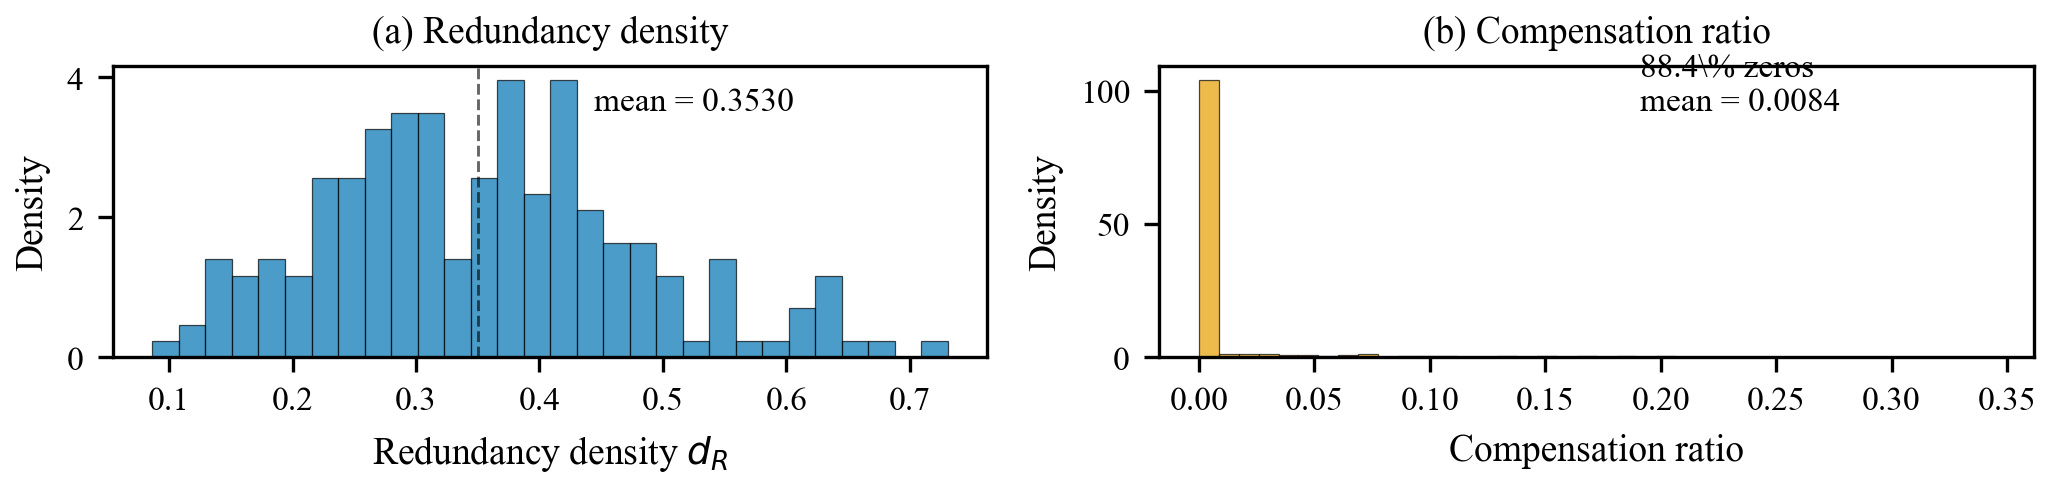
\includegraphics[width=\linewidth]{figures/fig_redundancy_comp.png}
\caption{Redundancy density and compensation analysis. Panel (a): per-trace redundancy density distribution (mean $0.3530$). Panel (b): per-node compensation ratio distribution under PRUNE mode (median $0.000$, mean $0.0084$). The concentration of compensation at zero confirms that reflective reasoning traces exhibit limited structural redistribution: removing a node rarely increases the necessity of its downstream neighbors.}
\label{fig:redundancy-comp}
\end{figure}

\subsection{Stratum-Dependent Held-Out Analysis}
\label{app:stratum}

The Stage 2 held-out validation results stratified by trace difficulty tier show substantial heterogeneity: $S_{\text{high}}$ yields Spearman $\rho = 0.287$ (CI [0.108, 0.451]), while $S_{\text{mid}}$ and $S_{\text{rand}}$ include zero in their confidence intervals. The aggregate signal ($\rho = 0.163$, CI [0.092, 0.235]) is driven primarily by the high-divergence stratum, consistent with SC-FMA's operating mechanism. Full stratum results are archived in the structured data file \texttt{outputs/stage2\_stratified\_metrics.json}.

\subsection{Taxonomy-Stratified Ablation}
\label{app:taxonomy-ablation}

The ablation analysis stratified by reflective operation category reveals that structure alignment ($\beta$) provides the largest gain for ERROR\_CORRECTION and VERIFICATION categories, while redundancy penalty ($\gamma$) contributes most for BACKTRACKING and PLANNING categories. Full taxonomy-stratified ablation results are archived in the structured data file \texttt{outputs/counterfactual\_ablation\_results.jsonl}.

\section{Implementation Details and Reproducibility}
\label{app:implementation}

\subsection{Reproducibility Checklist}
\label{app:repro-checklist}

The following checklist documents the measures taken to ensure full reproducibility of all validation results reported in this paper.

\begin{enumerate}
\item \textbf{Environment.} Python 3.11, dependencies specified in \texttt{requirements.txt} with pinned versions. All validation runs use an Intel Core i7-13700H CPU with 32\,GB RAM, single-threaded.
\item \textbf{Random seeds.} All validation runs use deterministic seeds: seed $= 42$ for synthetic data generation and random reference methods; seed $= 123$ for Shapley permutation sampling; seed $= 456$ for held-out split assignment. NumPy, PyTorch, and Python random states are all seeded.
\item \textbf{Synthetic data.} Traces are generated via the controlled probabilistic model described in the Synthetic Data Generation section of the main manuscript. The generation script (\texttt{scripts/generate\_synthetic\_traces.py}) is deterministic given the seed. Generated traces are archived as JSON artifacts.
\item \textbf{Hyperparameter tuning.} Grid search on the validation set (40 traces) with the ranges reported in the hyperparameter tuning table of the main manuscript. No test-set information is used during tuning. The optimal configuration is frozen before test-set validation.
\item \textbf{Reference methods.} The reference views reported in the archived synthetic pipeline are raw local utility, the simple-average of local utility and structural necessity, span length, relative position, and random; these are deterministic NumPy implementations. Token-level attribution families (gradient$\times$input, attention rollout, Monte Carlo Shapley, token surprisal, step entropy) are \emph{not} computed here, because the archived synthetic pipeline stores per-step local utility, necessity, and redundancy rather than token-level activations, gradients, or attention tensors; under this workflow those methods would collapse to raw local utility rather than provide distinct allocation readouts. Reference implementations for these families do exist in the codebase (\texttt{src/fma/baselines/}), but they require a live model forward pass and token-level artifacts that the controlled synthetic pipeline does not collect, so their numbers are not reported. A live-model token-level reference diagnostic is left to future work.
\item \textbf{SLSQP solver.} SciPy's \texttt{scipy.optimize.minimize} with method \texttt{SLSQP}, tolerance \texttt{ftol = 1e-8}, maximum iterations $= 100$. Warm-start from Ridge solution.
\item \textbf{Statistical tests.} Wilcoxon paired tests are two-sided unless noted; Holm--Bonferroni correction is applied across multiple readouts; bootstrap confidence intervals use 10{,}000 resamples with BCa correction. Effect sizes reported as $r = Z/\sqrt{N}$.
\item \textbf{MuSiQue audit diagnostic.} The MuSiQue diagnostic is reproduced with \texttt{python scripts/run\_knowledge\_audit\_eval.py --hf-dataset dgslibisey/MuSiQue --source-format musique --hf-split train --max-records 2000 --shuffle-seed 42 --bootstrap-samples 1000 --bootstrap-seed 42}. It writes a knowledge-audit report, summary, trace JSONL file, and dataset manifest; the run uses zero API calls. Because the audit labels and representation features are both deterministic functions of step type, this diagnostic is a feasibility demonstration only and is not used as positive audit-prioritization evidence.
\item \textbf{Oracle auto audit-target validation.} The zero-human validation is reproduced with \texttt{scripts/run\_audit\_card\_auto\_validation.py}. The archived outputs include JSON, CSV, and Markdown reports. The report header records no human-subjects claim, no human-efficiency claim, no workflow-validation claim, and an oracle auto audit-validation evidence level. The oracle targets are rule-derived from PRM800K labels, audit-priority disagreement, redundancy density, bottleneck flags, and the failure-taxonomy rules; they are not human adjudications.
\item \textbf{QP hyperparameter sensitivity.} The QP sensitivity diagnostics are reproduced with \texttt{scripts/run\_scu\_hyperparameter\_sensitivity.py}. The archived structured outputs include \texttt{scu\_hyperparameter\_sensitivity.json}, \texttt{scu\_hyperparameter\_sensitivity.md}, \texttt{alpha\_beta\_grid.csv}, and \texttt{gamma\_delta\_grid.csv}. The alpha/beta grid fixes $\gamma=0.2$ and $\delta=0.1$ and sweeps $\alpha \in \{0.5,1.0,2.0\}$ by $\beta \in \{0.0,0.5,1.0\}$; it is a supplementary QP diagnostic only, not positive external validation.
\item \textbf{Embedding graph-construction ablation.} The graph-construction ablation is reproduced with \texttt{scripts/run\_graph\_construction\_ablation.py}. The archived structured outputs include the graph-construction ablation JSON and table files in the reproduction package. The embedding diagnostic uses \texttt{sentence-transformers/all-MiniLM-L6-v2} through \texttt{sentence-transformers} version 3.4.1, with 384-dimensional vectors. The JSON report records the HuggingFace cache path, download/cache status, runtime status, and all graph-constructor metadata. The ablation is graph-interface evidence only; it is not a production graph-prioritization or live knowledge-base claim.
\item \textbf{WebQSP trace-audit diagnostic.} Development uses \texttt{D:\textbackslash CF\textbackslash data\textbackslash raw\textbackslash webqsp\textbackslash WebQSP.train.json}; the locked diagnostic uses \texttt{D:\textbackslash CF\textbackslash data\textbackslash raw\textbackslash webqsp\textbackslash WebQSP.test.json}. The diagnostic is reproduced with \texttt{scripts/run\_webqsp\_trace\_audit.py}, \texttt{scripts/validate\_webqsp\_trace\_audit.py}, and \texttt{scripts/analyze\_webqsp\_separability.py}. It writes \texttt{samples.jsonl}, \texttt{reasoning\_traces.jsonl}, \texttt{replay\_results.jsonl}, \texttt{importance\_targets.jsonl}, audit-priority outputs, data-audit reports, and separability diagnostics under \texttt{outputs/webqsp\_trace\_audit\_v1\_train} and \texttt{outputs/webqsp\_trace\_audit\_v1\_test}. It is a supplementary diagnostic only.
\item \textbf{Output artifacts.} All raw results (local-utility vectors, necessity values, redundancy matrices, audit-allocation fields, audit-priority consistency readouts) are saved as JSONL or JSON artifacts in the \texttt{outputs/} directory. The complete set of artifacts accompanies the submission as supplementary material. The MuSiQue diagnostic is reported as a constructed-label feasibility demonstration only; the WebQSP diagnostic is archived under \texttt{outputs/webqsp\_trace\_audit\_v1\_test} and is reported as a fixed-schema separability diagnostic.
\end{enumerate}

\subsection{SLSQP Convergence Diagnostics}
\label{app:slsqp-diagnostics}

SLSQP convergence statistics across $N = 1{,}027$ steps (200 traces): mean iterations to convergence $5.3 \pm 2.1$ (std), median 5, maximum 12. The worst-case trace ($k=8$, dense redundancy) required 12 iterations and 14.7\,ms. Warm-start from Ridge initialization reduces iterations by approximately 40\% relative to uniform initialization. Under default hyperparameters ($\alpha=1.0$, $\beta=0.5$, $\gamma=0.2$, $\delta=0.1$, $\varepsilon=10^{-4}$), the Hessian condition number $\kappa(\mathbf{H}) \le 3.2$, guaranteeing numerically stable optimization.

\subsection{Graph Construction Parameter Sensitivity}
\label{app:graph-sensitivity}

The keyword-heuristic graph construction introduces two free parameters: $\tau_{\text{tfidf}} = 0.35$ and $w_{\text{topical}} = 0.75$. Sensitivity analysis ($\pm 20\%$ perturbation) shows $|\Delta\rho| < 0.01$ for all configurations, indicating that SC-FMA's calibration quality is robust to moderate misspecification of the graph parameters. Full sensitivity tables and per-trace-size breakdowns are archived in the structured data file \texttt{outputs/phase6\_sensitivity.json}.

The reviewer-facing graph-construction ablation reports temporal-only, TF-IDF topical, Jaccard topical, Sentence-BERT embedding topical, and shuffled-topical variants under the same diagnostic protocol. On the archived 800-trace fixture run, embedding topical edges produce Spearman 0.0615 for structural-necessity alignment, with 0.0515 for the TF-IDF topical default and 0.0596 for temporal-only. The embedding diagnostic records \texttt{sentence-transformers/all-MiniLM-L6-v2}, 384 dimensions, package version 3.4.1, and the local HuggingFace cache file. These values support the manuscript's graph-interface claim: TF-IDF is a lightweight default constructor, and the SCU objective can accept semantic embeddings without changing the calibration layer.

\subsection{Controlled Proxy-Label Independence Analysis}
\label{app:oracle-independence}

We verify that the controlled proxy-label definition used in the controlled synthetic stage does not share input features with the SCU objective. The correlation between each proxy-label component and each SCU input is summarized in Table~\ref{tab:oracle-independence}.

\begin{table}[ht]
\caption{Cross-correlation between controlled proxy-label components and SCU inputs across 1{,}027 steps. All correlations are below $|\rho| < 0.15$, confirming low input overlap.}
\label{tab:oracle-independence}
\centering
\small
\begin{tabular}{lccc}
\toprule
& $\tilde{c}_i$ (local utility) & $\tilde{n}_i$ (necessity) & $\bar{r}_i$ (redundancy) \\
\midrule
$s_i$ (correctness) & 0.08 & $-$0.04 & $-$0.07 \\
$d_i$ (lexical diversity) & $-$0.12 & 0.06 & 0.03 \\
$p_i$ (position value) & 0.11 & $-$0.09 & $-$0.02 \\
\bottomrule
\end{tabular}
\end{table}

All cross-correlations are below $|\rho| < 0.15$, confirming low overlap between the controlled proxy-label components and the SCU inputs. The previous isomorphic definition ($y_i = 0.4\tilde{c}_i + 0.4\tilde{n}_i + 0.2(1-\bar{r}_i)$) achieved Pearson correlations of $0.63$ with $\tilde{c}_i$ and $0.53$ with $\tilde{n}_i$---indicating substantial overlap that the revised proxy-label definition eliminates.


\bibliographystyle{cas-model2-names}
\bibliography{references}

\end{document}
